\section{String matching with finite automata}

\begin{frame}
\begin{dfn}[automata]
    finite automaton은 다음과 같이 5개의 튜플로 구성된다.
    \begin{itemize}
        \item $Q$ : 유한 상태의 집합
        \item $q_0$ :시작 상태 ($q_0 \in Q$)
        \item $A$ : 받아들이는 상태의 구분된 상태 ($A \subset Q$)
        \item $\Sigma$ : 유한 입력 알파벳 집합
        \item $\delta$ : $Q \times \Sigma$에서 $Q$로 매핑되는 전이 함수 $M$    \end{itemize}
\end{dfn}
\end{frame}

\begin{frame}
    
뭔소린지모르겠죠?

저도 그럼

오토마타 내용 통째로 생략
\end{frame}

\begin{frame}[$\delta$ 상태표란]
    \begin{itemize}
        \item 문자열 $T$는 각 자리마다 상태를 가진다.
        \item 초기 시작 상태는 0
        \item 현재 문자의 상태는 문자의 상태와 현재 문자에 따라 정해진다.
        \item 상태는 상태표를 보고 정한다.
    \end{itemize}
\end{frame}


\begin{frame}[$\delta$ 상태표를 구해라]
    \begin{enumerate}
        \item 상태 : 앞에서부터 각각의 문자가 가장 길게 일치하는 갯수
        \item $(m+1) \times \Sigma$ 배열
        \item 상태가 $m$에 도달하면 매칭
    \end{enumerate}
\end{frame}

\begin{frame}
    \begin{figure}[h!]
        \centering
        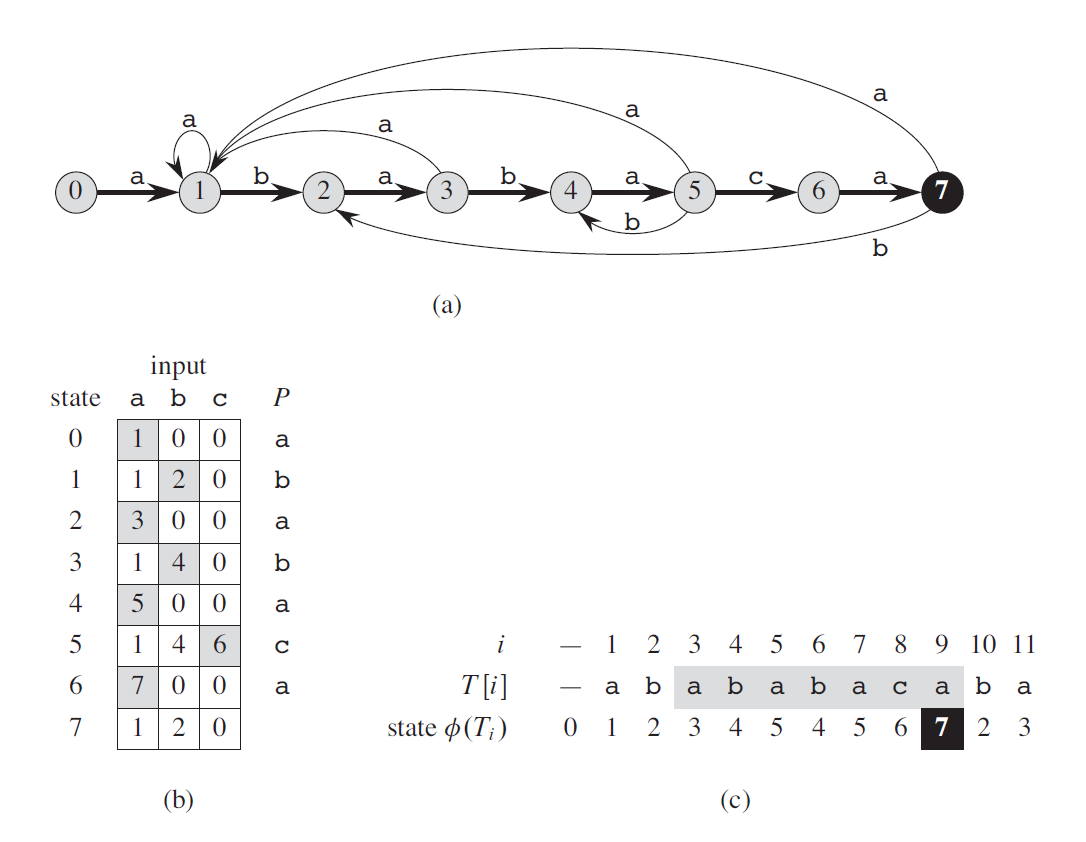
\includegraphics[scale=0.4]{pic2.PNG}
        \caption{$|\Sigma|  = 3$ ``a,b,c", $m = 7$
    \end{figure}
\end{frame}

\begin{frame}
    \begin{lstlisting}[style = CStyle]
    FINITE-AUTOMATON-MATCHER(T, delta , m)
    n = T.length
    q = 0 
    for i = 1 to n
        q = d(q,T[i])
        if q == m
            print ``Pattern occurs with shift i-m"
    \end{lstlisting}
\end{frame}


\begin{frame}
    
\end{frame}

    


\begin{frame}
\begin{lstlisting}[style = CStyle]
    COMPUTE-TRANSITION-FUNCTION(P, Sigma)
    m = P.length
    for q = 0 to m
        for a in Sigma
            k = min(m+1,q+2)
            repeat 
                k = k - 1
                until P_k ] P_q-a
                d(q,a) = k
    return d
\end{lstlisting}
\end{frame}


상태표를 구하기위해서 다음과 같이 진행한다.
각 상태 $q$ 마다 각 알파벳 $a$를 뽑는다.
현재 상태 $q$의 문자열 + 'a'가 임의의 상태 $k$를 끝에서 포함하는지 검사하고 다를시 $k$를 계속 낮춰간다.


\begin{frame}
    \begin{itemize}
        \item 전처리의 수행시간 $O(m^3 \Sigma)$
        \item 상태표의 공간 복잡도의 크기가 $\Theta(m|\Sigma|)$
        \item $\Theta(n)$
    \end{itemize}
\end{frame}

\begin{frame}
    \begin{itemize}
        \item 뒷절의 $KMP$방식을 차용해서 전처리 시간을 $O(m \Sigma)$로 개선할수있다.
        \item 공간 복잡도의 크기를 더 줄여보자.    
    \end{itemize}
\end{frame}



\section{The KMP algorithm}

\begin{frame}[KMP?]
    \begin{itemize}
        \item Knuth-Morris-Pratt이 공동 발표한 알고리즘
    \end{itemize}
\end{frame}

\begin{frame}[$\delta$대신 $\pi$]
    \begin{itemize}
        \item 크기 $m$
        \item 매칭이 실패했을때 사용.
        \item 앞의 문자열과 가장 근접하게 일치하는 위치를 반환
    \end{itemize}
\end{frame}

\begin{frame}
\begin{figure}[h!]
    \centering
    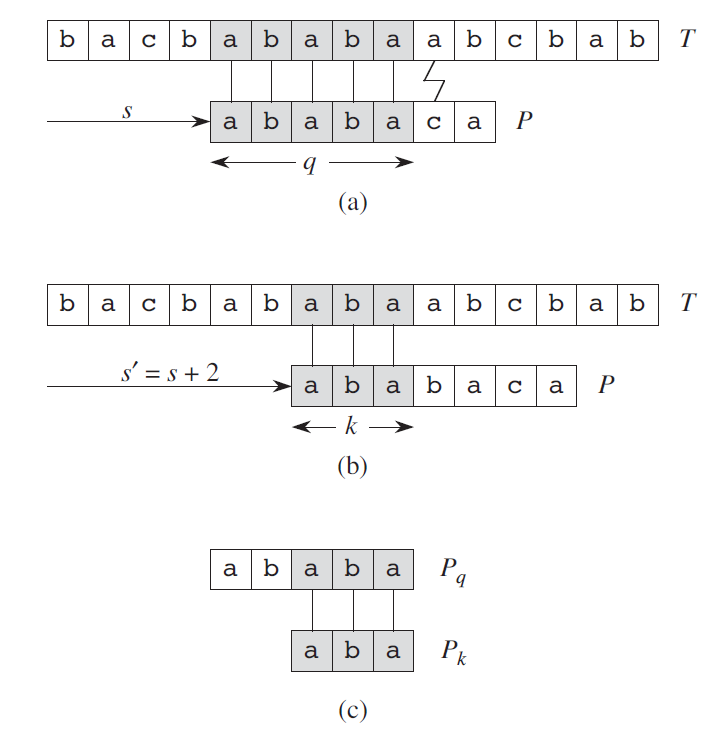
\includegraphics[scale=0.7]{pic3.PNG}
    %\caption{}
\end{figure}
\end{frame}

\begin{frame}
\begin{figure}[h!]
    \centering
    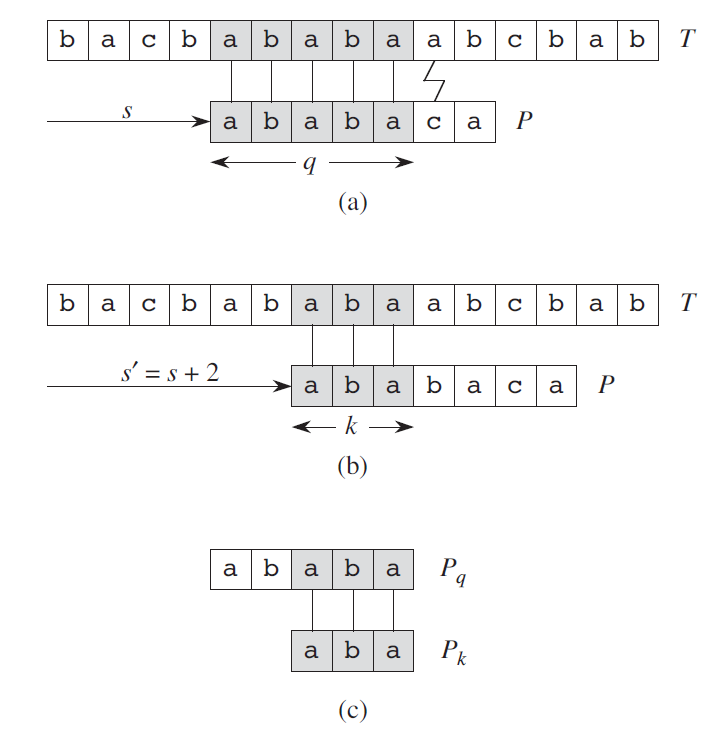
\includegraphics[scale=0.7]{pic3.PNG}
    %\caption{}
\end{figure}

\end{frame}


\begin{frame}
\begin{figure}[h!]
    \centering
    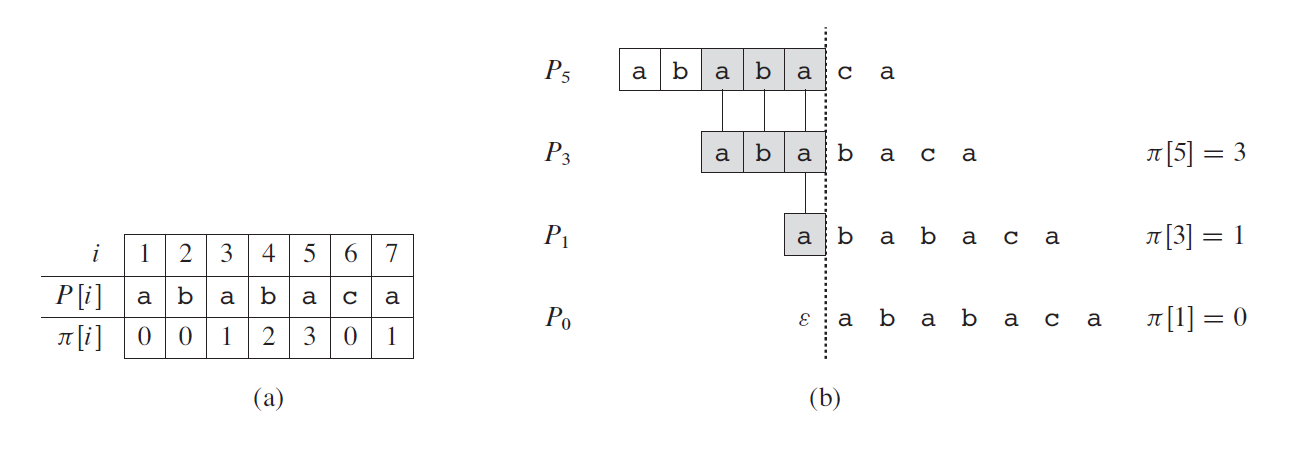
\includegraphics[scale=0.4]{pic4.PNG}
    \caption{(a)는 패턴 $P$와 전처리한 $\pi[1..7]$ (b)는 $P[5]$에서 다음 문자가 매칭이 틀렸을때 그에 따른 $\pi$값과 되돌아가는 순서를 나타낸것이다.}
\end{figure}

\begin{frame}
\begin{lstlisting}[style = CStyle]
KMP-MATCHER(T,P)
    n = T.length
    m = P:length
    PI[] = COMPUTE-PREFIX-FUNCTION(P)
    q = 0 // number of characters matched
    for i = 1 to n // scan the text from left to right
        while q>0 and P [q+1] != T[i]
            q = PI[q] // next character does not match  
        if P [q+1] == T[i]
            q = q + 1 // next character matches
        if q == m // is all of P matched?
            print ``Pattern occurs with shift" i - m
            q  = PI[q]
\end{lstlisting}
\end{frame}




\begin{frame}
\begin{lstlisting}[style = CStyle]
COMPUTE-PREFIX-FUNCTION(P) /
m = P.length
let PI[1..m] be a new array
PI[1] = 0
k = 0
for q = 2 to m
    while k>0 and P[k+1] != P[q]
        k = P[k]
    if P[k+1] == P[q]
            k = k + 1
    PI[q] = k 
retunr PI
\end{lstlisting}

\end{frame}
\begin{itemize}
    \item 전처리 : $O(m)$
    \item 매칭시간 : $\Theta(n)$
\end{itemize}
\end{frame}

%http://yoonkn.blogspot.com/2009/06/beamer-에서-table-쓰기-한프레임안에-큰테이블-구겨넣기.html
\begin{frame}[정리]



    \item 전처리의 수행시간 $O(m^3 \Sigma)$
    \item 상태표의 공간 복잡도의 크기가 $\Theta(m|\Sigma|)$
    \item $\Theta(n)$
    
    전처리 : $O(m)$  매칭시간 : $\Theta(n)$
\end{frame}
